\section{Method}
\label{sec:method}

This section describes our approach to solving the page rank estimation problem. We present our methodology as we have applied it to the problem at hand, as opposed to extracting the generic, underlying principles, as these are mostly covered in the background section of this document.

The page rank estimation problem is, given a webpage represented as an attributed graph with screenshots, to estimate the global popularity of that webpage.
Our ground-truth for \textit{popularity} is a list containing 100,000 webpages, created by Open PageRank.
More details can be found in Section~\ref{OpenPageRank}.
The given data has several characteristics which have influenced our way of tackling the problem:

\begin{itemize}
    \item With approximately 100,000 samples, there is plenty of data available. Each sample, i.e. a domain, is made up of up to 16 images (eight desktop and eight mobile screenshots).
    \item The problem is a ranking task. Samples need to be ordered and during inference the rank of a (possibly) unseen sample must be predicted. Besides the webpage ranking list (containing rank and domain) there is no information available.
    \item Images make up the majority of the information contained in the dataset. Neural networks, in particular convolutional neural networks (CNNs; see \cite{lecun1989backpropagation}) are performing well at processing images and at extracting features from them. With \cite{krizhevsky:imagenet} they have become the de-facto standard way of solving image classification problems where ever large datasets are available.
    \item The samples are variably-sized and can be easily represented as a graph: The number of screenshots taken from a domain may vary depending on the number of subpages. Links between subpages can be represented as edges in a graph. Naturally, the samples can be seen as graphs and a model capable of using the entire information from the graph seems best suited.
    \item The data is relatively inconsistent, e.g. samples might be mostly black or ranks might be inaccurate, as the global page ranking list is subject to change over time.
\end{itemize}

Motivated by the stated observations, we use a combination of CNN and graph network (GN), trained with ranking loss functions, to predict page ranks.

Learning features as opposed to hand-engineering them seems reasonable, because it is unknown to us what the visual elements are that distinguish popular and unpopular webpages and whether they exist at all. Until this point is is unknown to us whether it is feasible to predict a domain's rank based on the visual appearance of its web pages. A dataset containing more than 1,000,000 images provides enough training data to work with high-capacity, deep models, capable of learning complex features.

CNNs are the most common choice for image processing in the deep learning domain. While many of today's CNN-papers deal with natural images, e.g. \cite{gu2018ava,szegedy2017inception,openai:learningdexterity}, there have been applications with computer generated images as well: \cite{beltramelli:pix2code} converts a screenshot into a fixed size feature vector to infer the design layout of given user interface from a screenshot. This work as well as the general attention CNNs get indicate that they are a suitable choice for web page screenshot processing and feature extraction.

Graph networks are designed to process graphs, possibly ones where a node's attribute is an image. Graph networks naturally scale to graphs of arbitrary size and type of content present in the graph. While processing the graph, information can flow between nodes (message passing). While we focus on visual information (screenshots) of websites, future extensions could augment nodes with textual or other data as well.

Ranking problems are a well studied field and losses for different setups have been defined in previous works. We incorporate in particular the probabilistic ranking loss by \cite{Burges:learningtorankwithsgd} into our model.

We define an accuracy metric that allows us to evaluate the performance of our model. It measures how accurately the model ranks any two given webpages from a subset of the dataset relative to each other. This accuracy metric is also the primary way of comparing models to each other, e.g. for hyperparameter tuning.

While our dataset contains webpages from domains which are (or have been) publicly available on the web, we want it to work with unseen inputs as well. The goal of our model's inference mode is to either estimate the absolute popularity of a webpage with respect to the top 100,000 webpages or, secondly, compare two (or more) given webpages relative to one and another.

\begin{figure}
    \centering

    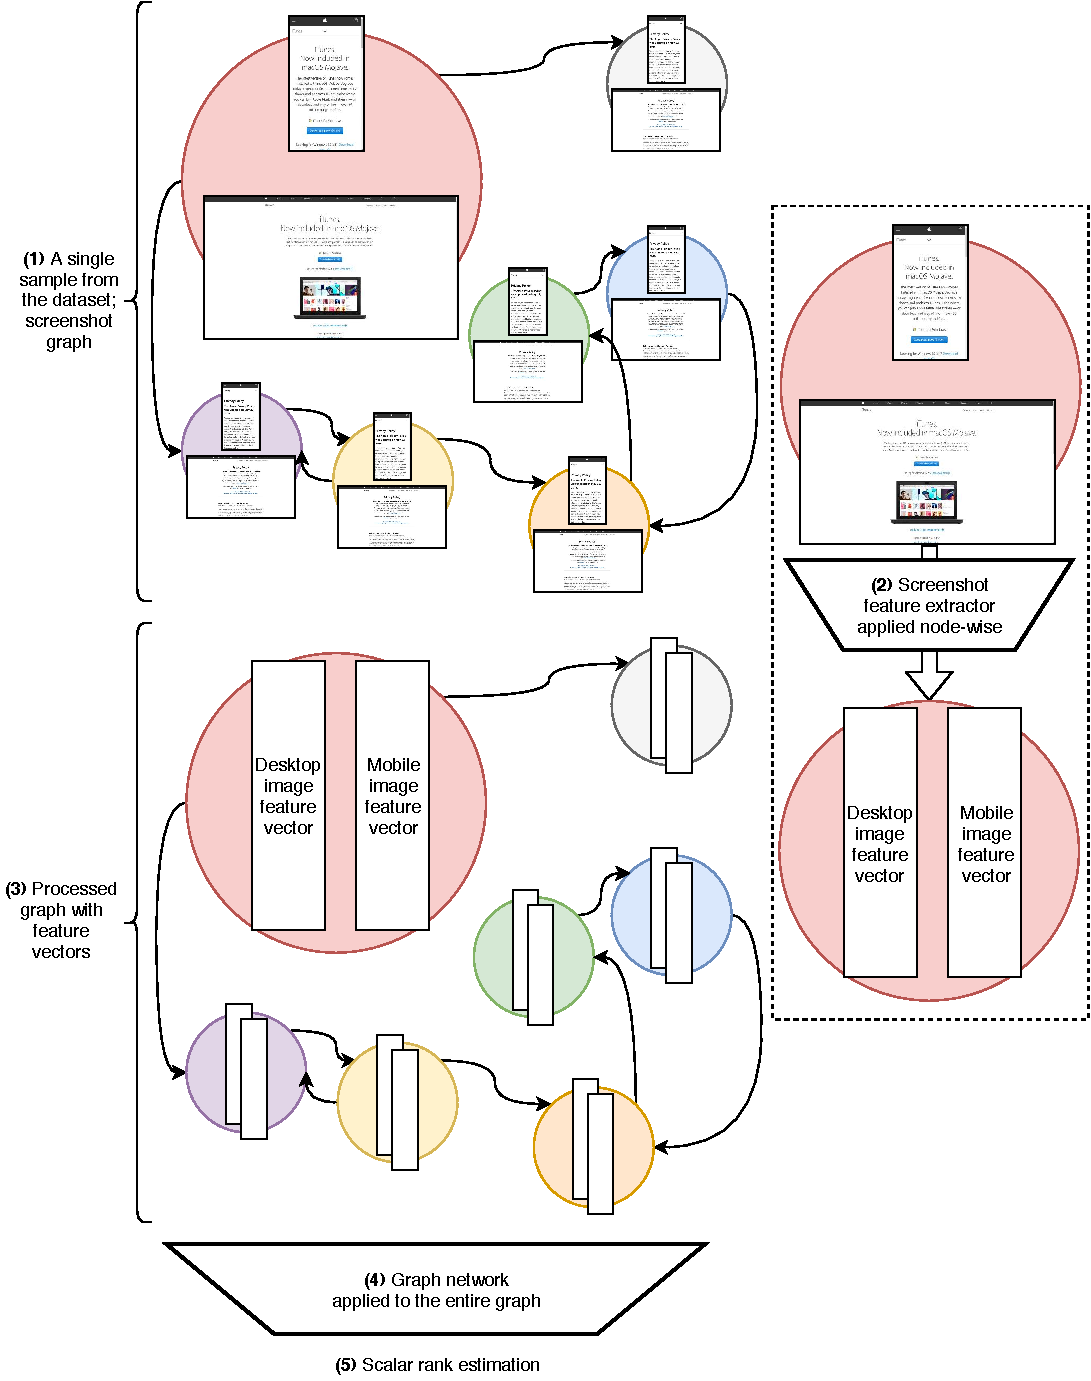
\includegraphics[scale=0.55]{resources/model-architecture}
    \caption[Illustration of the model processing pipeline]{Illustration of the web page rank estimation model processing pipeline. Input to the model is a graph representing the web pages of a domain (1). Each node is attributed with two screenshots and the nodes are interconnected by web links. A screenshot feature extractor CNN is (2) applied node-wise, thereby converting the screenshot graph into a graph with feature vectors (3). The feature vector graph is the input to a (4) graph network which looks at the graph as a whole (as opposed to node-wise processing). It compresses the graph into a single scalar (5) from which the relative ranking can be inferred.\\
    The internals of module (2) are explained in Section~\ref{sec:screenshotfeatextr}; the ones of (4) in Section~\ref{sec:gnblocks}.}
    \label{fig:methodcomponents}
\end{figure}

The remainder of this section describes the components of our model in greater detail; Figure~\ref{fig:methodcomponents} gives an overview of the model's internal processing pipeline. We also introduce our loss function and the evaluation metric we use to measure the performance of our model. The dataset is described separately in Section~\ref{sec:datasets}.

\subsection{Screenshot Feature Extractor}
\label{sec:screenshotfeatextr}

The screenshot feature extractor is an integral component of the model. Its task is to extract a vector of fixed size from a given website screenshot. The vector is supposed to contain a condensed version of the information contained in the original image. Condensed with respect to the specific task the feature extractor is trained on.

The idea of feature extraction is a reoccurring scheme in the field of deep learning. Recurrent neural networks such as LSTMs (\cite{hochreiter1997lstm}) can extract a fixed size vector from a variable length sequence, used e.g. to map a sentence into a representation space \cite{salesforceabstractivesummarization}. Similarly, CNNs are used to extract features from images: It is a common architectural choice to classify an image with a CNN, the feature extraction, followed by fully connected layers, referred to as classification head, see e.g. \cite{krizhevsky:imagenet,Girshick15:fastrcnn,szegedy2017inception}. We borrow this idea and extract feature vectors from screenshots, which are the input to our model. The extracted features serve as input to the following stage, a graph network.

Mathematically, a screenshot feature extractor is a function mapping a screenshot into a smaller vector space of dimensionality $d_\text{featvec}$: $f:\mathbb{R}^{480\times270\times3}\rightarrow\mathbb{R}^{d_\text{featvec}}$. We are working with two different types of screenshots, namely desktop and mobile webpage screenshots. The screenshots are similar in that they contain similar content (a website), however, potentially of different size. Also, mobile screenshots might have a different look overall, commonly having a menu drawer in the corner and a single-column layout. We decide to process a tuple of corresponding mobile and desktop screenshots with a single function to share some of the function's parameters. Specifically, the employed feature extractor is a function \begin{equation}
f_\text{dm}:\left(\mathbb{R}^{480\times270\times3},\mathbb{R}^{187\times333\times3}\right)\rightarrow\left(\mathbb{R}^{d_\text{featvec}},\mathbb{R}^{d_\text{featvec}}\right)\,,
\end{equation} where \enquote{dm} stands for desktop-mobile. The input tensors are two screenshots (desktop and mobile respectively), with three color channels. The output is a tuple consisting of two vectors. They are supposed to be mappings of the screenshot into a $d_\text{featvec}$-dimensional feature space.

\begin{figure}
    \centering
    \begin{tikzpicture}[>=stealth, thick]
    \node (I_d) at (2,-16) [draw, process, align=flush center]
        {Desktop screenshot\\$\tens{I}_\text{d}\in\mathbb{R}^{480\times270\times3}$};
    
    \node (I_m) at (6,-16) [draw, process, align=flush center]
        {Mobile screenshot\\$\tens{I}_\text{m}\in\mathbb{R}^{187\times333\times3}$};
    
    \node (block1_d) at (2,-14) [draw, double, align=flush center]
    {Block1\_d\\$n_\text{filters}=32$};

    \node (block1_m) at (6,-14) [draw, double, align=flush center]
    {Block1\_m\\$n_\text{filters}=32$};

    \node (block2_d) at (2,-12) [draw, double, align=flush center]
    {Block2\\$n_\text{filters}=64$};
    \node (block2_m) at (6,-12) [draw, double, align=flush center]
    {Block2\\$n_\text{filters}=64$};

    \node (block3_d) at (2,-10) [draw, double, align=flush center]
    {Block3\\$n_\text{filters}=128$};
    \node (block3_m) at (6,-10) [draw, double, align=flush center]
    {Block3\\$n_\text{filters}=128$};

    \node (block4_d) at (2,-8) [draw, double, align=flush center]
    {Block4\\$n_\text{filters}=256$};
    \node (block4_m) at (6,-8) [draw, double, align=flush center]
    {Block4\\$n_\text{filters}=256$};

    \node (dense_d) at (2,-6) [draw, double, align=flush center]
    {Dense\\$n_\text{units}=256$};
    \node (dense_m) at (6,-6) [draw, double, align=flush center]
    {Dense\\$n_\text{units}=256$};

    \node (dense2_d) at (2,-4) [draw, double, align=flush center]
    {Dense\_d\\$n_\text{units}=d_\text{featvec}$};
    \node (dense2_m) at (6,-4) [draw, double, align=flush center]
    {Dense\_m\\$n_\text{units}=d_\text{featvec}$};

    \node (feat_d) at (2,-2) [draw, process, align=flush center]
        {Desktop feature vector\\$\bm{x}_\text{d}\in\mathbb{R}^{d_\text{featvec}}$};
    
    \node (feat_m) at (6,-2) [draw, process, align=flush center]
        {Mobile feature vector\\$\bm{x}_\text{m}\in\mathbb{R}^{d_\text{featvec}}$};
    
    \draw[->] (I_d) -- (block1_d);
    \draw[->] (I_m) -- (block1_m);

    \draw[->] (block1_d) -- (block2_d);
    \draw[->] (block1_m) -- (block2_m);
    \draw[dashed,<->] (block2_m) -- (block2_d);

    \draw[->] (block2_d) -- (block3_d);
    \draw[->] (block2_m) -- (block3_m);
    \draw[dashed,<->] (block3_m) -- (block3_d);

    \draw[->] (block3_d) -- (block4_d);
    \draw[->] (block3_m) -- (block4_m);
    \draw[dashed,<->] (block4_m) -- (block4_d);

    \draw[->] (block4_d) -- (dense_d);
    \draw[->] (block4_m) -- (dense_m);
    \draw[dashed,<->] (dense_m) -- (dense_d);

    \draw[->] (dense_d) -- (dense2_d);
    \draw[->] (dense_m) -- (dense2_m);

    \draw[->] (dense2_d) -- (feat_d);
    \draw[->] (dense2_m) -- (feat_m);
    
    \end{tikzpicture}
    \caption[Illustration of the feature extractor]{Illustration of the feature extractor $f_\text{dm}$; inputs are at the bottom, outputs at the top. Blocks with double borders are parameterized, dashed arrows indicate parameter sharing. The weight sharing between inner layers allows for similar, yet different feature extraction because the weight matrices of the first convolutional block and the last dense block are not shared.}
    \label{fig:featextr}
\end{figure}

We model the function $f_\text{dm}$ with a CNN. The high-level architecture is described and visualized in Figure~\ref{fig:featextr}. Each \textbf{Block} consists of the following components:
\begin{enumerate}
    \item 2D convolutional layer with $n_\text{filters}$ filters, preserving the spatial size of the tensor and increasing the number of channels.
    \item ReLU activation function, $\operatorname{relu}(x)=\max(0,x)$.
    \item Second 2D convolutional layer with $n_\text{filters}$ filters, preserving the size of the tensor along all dimensions.
    \item ReLU activation function.
    \item 2D max-pooling with a kernel size of $(3,3)$. This reduces the spatial size of the tensor by a factor of $3$ along both, width and height.
    \item 2D dropout (\cite{srivastava2014:dropout}) with drop probability $p_\text{drop}$, enabled during training, disabled during evaluation and inference.
\end{enumerate}
Exceptions to this are the first block which has a max-pooling size of $(2,2)$ and the fourth block which is followed by global average pooling. These deviations from \cite{beltramelli:pix2code} are made to account our specific screenshot dimensionality which varies from desktop to mobile.

The \textbf{Dense} blocks each contain a fully connected layer followed by ReLU activation and dropout. The last layer outputs the raw result of the matrix multiplication, without activation or dropout.

The parameters of the feature extraction model can be trained with backpropagation. The following modes of training are conceivable:
\begin{itemize}
    \item \textbf{End-to-end training [e2e]}. The feature extractor is trained alongside with the other components of the model, gradients are computed by backpropagating through the following components. This method will train the CNN such that the extracted vectors contain features most helpful/relevant for the overall task. The downside is the additional computational complexity introduced by backpropagating through a graph network.
    \item \textbf{Pre-training without fine-tuning [woft]}. The weights of the feature extractor are learned on a separate auxiliary task and transferred to be used for the actual problem. This method requires an auxiliary task, which (in this setting) may be the prediction of a page rank based solely on a single desktop-mobile screenshot tuple. If the model parameters are kept frozen, i.e. are not being fine-tuned, the feature vectors for the dataset can be cached, once the entire model is trained on the main task. That way the computational overhead of passing images through the CNN can be omitted, greatly increasing the training speed and decreasing GPU memory requirements. Even though the described auxiliary task is similar to the page rank prediction based on an entire graph of screenshots, its difference may lead to slightly less meaningful feature vectors.
    \item \textbf{Pre-training with fine-tuning [wft]}. Same as \textit{pre-training without fine-tuning} except the weights are kept trainable and are fine-tuned on the main task as well. Caching of feature vectors is not possible.
\end{itemize}

\subsection{Graph Network Blocks}
\label{sec:gnblocks}

After converting the graph of screenshots into a graph of feature vectors, the entire graph is fed into the graph network (GN); component (4) in Figure~\ref{fig:methodcomponents}. The GN module is an integral component of our model: It utilizes the graph structure of the dataset samples and outputs the actual model prediction, thereby converting a graph into a continuous scalar, interpretable as a rank estimation.

The GN consists of several GN blocks, which were introduced in \cite{deepmind:graphnets}. A summary of the most important aspects as well as the notation we use in the following can be found in Section~\ref{sec:graphnetworks}.

Formally, the GN module converts a graph into a scalar, i.e. \begin{equation}
    \label{eq:gnmodule}
    f_\text{gn}:\mathbb{G}\rightarrow\mathbb{R}\,,
\end{equation} where $\mathbb{G}$ denotes the set of all possible graphs. The input graph represents a website and consists of up to eight nodes. Each node contains two feature vectors which are the screenshot feature extractor's output. The directed edges point from nodes to nodes which contain hyperlinks. Initially, the edges are (opposed to the nodes which contain feature vectors) not attributed.

On a semantic level the GN module consists of three different types of blocks: encoder, core, and decoder. For each of these blocks variants can be used but the role remains the same. This idea is dubbed \textit{encode-process-decode} and depicted in Figure~\ref{fig:gn-enc-proc-dec}.

Our \textbf{encoder block} $\text{GN}_\text{enc}$ converts the raw input graph into a homogeneous graph where nodes, edges, and global state are all attributed with a single vector. In our case this is achieved by defining the following update and aggregation functions for the encoder:\begin{align}
    \phi^e_\text{enc}\left(\bm{e}_k,\bm{v}_{r_k},\bm{v}_{s_k},\bm{u}\right)=&\bm{v}_{s_k}\label{eq:enc:edgeupdate}\\
    \rho^{e\rightarrow u}_\text{enc}\left(\mathbb{E}'\right)_j=&\operatorname{avg}\left(\left\{x_j:\bm{x}\in\mathbb{E}'\right\}\right)\label{eq:enc:edgeaggreforu}\\
    \phi^v_\text{enc}\left(\bm{\overline{e}}'_i,\bm{v}_i,\bm{u}\right)=&\bm{v}_i\label{eq:enc:nodeupdate}\\
    \phi^u_\text{enc}\left(\bm{\overline{e}}',\bm{\overline{v}},\bm{u}\right)=&\bm{\overline{e}}'\label{eq:enc:uupdate}\,,
\end{align}where $\rho^{e\rightarrow v}$ and $\rho^{v\rightarrow u}$ remain undefined because they are not needed. The edges are initially populated with the feature vector of the sender node (Equation~\ref{eq:enc:edgeupdate}). Equation~\ref{eq:enc:edgeaggreforu}, the edge aggregation for the global state, is an element-wise averaging of the edge vectors. To ensure there is at least one element in $\mathbb{E}'$ we add reflexive edges to the graph so every node has at least one outgoing (and incoming) edge, namely the one pointing to itself. The node attributes remain unchanged, Equation~\ref{eq:enc:nodeupdate} is an identity mapping. The global state is set to be the aggregation of all edges (Equation~\ref{eq:enc:uupdate}). Alternatively, the node aggregation $\bm{\overline{v}}$ could be chosen; both options are equally valid and we did not perform experiments comparing both options within the scope of this work.

Intuitively, the encoder block can be seen as a preparation stage. It transforms the graph into the desired state and adds missing attributes. In fact, the entire feature extractor can be seen as an encoder block, too: It is a node-wise application of the CNN: $\phi^v_\text{core}\left(\bm{\overline{e}}'_i,\bm{v}_i,\bm{u}\right)=f_\text{dm}(\bm{v}_i)$, where $\bm{v}_i$ is a tuple made up of desktop and mobile screenshot. We chose not to formulate the overall model that way to aid understanding, but it illustrates the expressive power of the GN framework.

Before applying the encoder block we concatenate desktop and mobile feature vectors so node attributes are a single vector $\bm{v}=\begin{bmatrix}\bm{x}_\text{d} & \bm{x}_\text{m}\end{bmatrix}$.

Our \textbf{core block} $\text{GN}_\text{core}$ performs the graph \textit{understanding} part by performing the \textit{message passing} (see Section 4.3 in \cite{deepmind:graphnets}). It may be stacked $M$ times. 

We choose the aggregation functions $\rho^{e\rightarrow v}\left(\mathbb{E}'_i\right)$, $\rho^{e\rightarrow u}\left(\mathbb{E}'\right)$, $\rho^{v\rightarrow u}\left(\mathbb{V}'\right)$ to average the vectors element-wise, analogous to Equation~\ref{eq:enc:edgeaggreforu}. Alternatively, max-pooling could be used; we did not perform experiments comparing both options within the scope of this work.

The update functions for node attribute, edge attributes, and the global state are fully-connected layers with bias, followed by a ReLU activation function ($\operatorname{ReLU}(x) = \max(0,x)$) and dropout (see \cite{srivastava2014:dropout}; denoted by the function $\operatorname{drop}(\cdot)$). The exact definitions are the following:
\begin{align}
    \phi^e_\text{core}\left(\bm{e}_k,\bm{v}_{r_k},\bm{v}_{s_k},\bm{u}\right)=&
        \operatorname{drop}\left(\operatorname{ReLU}\left(
            \bm{W}_e\begin{bmatrix}\bm{e}_k & \bm{v}_{r_k} & \bm{v}_{s_k} & \bm{u}\end{bmatrix}^\mathsf{T}+\bm{b}_e
        \right)\right)\\
    \phi^v_\text{core}\left(\bm{\overline{e}}'_i,\bm{v}_i,\bm{u}\right)=&
        \operatorname{drop}\left(\operatorname{ReLU}\left(
            \bm{W}_v\begin{bmatrix}\bm{\overline{e}}'_i & \bm{v}_i & \bm{u}\end{bmatrix}^\mathsf{T}+\bm{b}_v
        \right)\right)\\
    \phi^u_\text{core}\left(\bm{\overline{e}}',\bm{\overline{v}},\bm{u}\right)=&
        \operatorname{drop}\left(\operatorname{ReLU}\left(
            \bm{W}_u\begin{bmatrix}\bm{\overline{e}}' & \bm{\overline{v}} & \bm{u}\end{bmatrix}^\mathsf{T}+\bm{b}_u
        \right)\right)\,,
\end{align}where $\begin{bmatrix}\cdot\end{bmatrix}$ denotes concatenation into a row vector. The core block can be repeated $M$ times. The trainable weight matrices $\bm{W}$ and biases $\bm{b}$ may either be shared between the $M$ core block replicas or different matrices/vectors can be used.

Our \textbf{decoder block} $\text{GN}_\text{dec}$ converts the graph returned from the last core block into the desired output. In our case the output of the GN module is a scalar (see Equation~\ref{eq:gnmodule}). We extract a scalar from the graph by muliplying the global state vector $u$ of the last core block with a weight vector of matching size and add a bias:
\begin{equation}
    \label{eq:dec:nodeupdate}
    \phi^u_\text{dec}\left(\bm{\overline{e}}',\bm{\overline{v}},\bm{u}\right)=\bm{w}_\text{dec}\cdot\bm{u}+\bm{b}_\text{dec}\,.
\end{equation}
The trainable parameters are $\bm{w}_\text{dec}$ and $\bm{b}_\text{dec}$.

Intuitively, the global state can be understood as an aggregation of the information contained in the graph. This is an elegant solution to the problem of converting a set into a vector, which must be solved when converting a graph of variable size into a single scalar.

\subsection{Loss Function}
\label{sec:loss}

Our model is trained with gradient descent which requires the definition of a loss function. We choose a probabilistic loss function, suitable for ranking problems, that is heavily inspired by \cite{Burges:learningtorankwithsgd}. We recap their approach as well as more information on ways of tackling ranking problems in our Section \textit{Learning to Rank} (\ref{sec:learningtorank}).

Let $\mathbb{D}=\left\{\left(G^{(i)},r^{(i)}\right)\right\}_{i=1}^N$ denote a dataset consisting of $N\ge2$ graphs and corresponding ranks.
Let $f_\text{model}(G)=\left(f_\text{dm}\circ f_\text{gn}\right)\left(G\right)$ be the model function mapping a graph to a scalar in $\mathbb{R}$.
$\bm{f}\in\mathbb{R}^N$ is the vector induced by applying the model function to the entire dataset:
\begin{equation}
    f_i=f_\text{model}\left(G^{(i)}\right)\,.
\end{equation}

Given the samples with indices $i$ and $j$, we interpret the model output as follows:
\begin{align}
    f_i>f_j&\implies G^{(i)}\triangleright G^{(j)}&G^{(i)}\text{ is higher ranked,}\\
    f_i<f_j&\implies G^{(i)}\triangleleft G^{(j)}&G^{(j)}\text{ is higher ranked,}\\
    f_i=f_j&\implies G^{(i)}\equiv G^{(j)}&\text{equal rank.}
\end{align}

All pairwise predictions (how the model ranks any two samples relative to each other) are stored in the matrix $\bm{O}\in\mathbb{R}^{N\times N}$, whose entries are defined as
\begin{equation}\label{eq:outputmatrix}
    O_{i,j}=f_i-f_j\,.
\end{equation}

The ground truth matrix $\bm{P}\in\mathbb{R}^{N\times N}$ can be derived from the data. $\bm{P}$ stands for probability. Its entries\begin{equation}\label{eq:groundtruthmatrix}
    P_{i,j}=\begin{cases}
        0&\text{if }r^{(i)}\triangleleft r^{(j)}\\
        0.5&\text{if }r^{(i)}\equiv r^{(j)}\\
        1&\text{if }r^{(i)}\triangleright r^{(j)}
    \end{cases}
\end{equation}indicate the probability of $r^{(i)}$ to be a higher rank (e.g. \#5) than $r^{(j)}$ (e.g. \#100). Note that a greater rank number is a lower rank; the highest rank is \#1. This can be confusing from time to time, we use the wording of a \textit{higher rank} to be a lower number, which is a higher position in the ranking.

The loss is defined as
\begin{equation}
    \label{eq:loss}
    \frac{1}{N^2}\sum_{i=1}^N\left(
        w_b\left(r^{(i)}\right)\sum_{j=1}^N
            \underbrace{\left(-P_{i,j}O_{i,j}+\log\left(1+e^{O_{i,j}}\right)\right)}_{C_{i,j}}
    \right)\,,
\end{equation}where $w_b:\mathbb{N}\rightarrow\mathbb{R}$ is a rank-dependent weighting function, which is explained below. The loss term can be understood as a computation of the pairwise loss for each pair of samples in the dataset, denoted by $C_{i,j}$. The leading factor $\frac{1}{N^2}$ normalizes so the number of samples $N$ does not affect the loss magnitude.

The loss asymptotes to a linear function. According to \cite{Burges:learningtorankwithsgd}, this is likely to be more robust with noisy labels than a quadratic cost. This behavior is illustrated in Figure~\ref{fig:costfn}.

We introduce the additional weighting factor
\begin{equation}\label{eq:weightingfactor}
    w_b(r)=1-\left(\frac{\log\left(r\times r_\text{max}\right)}{\log r_\text{max}}-1\right)^b\,,
\end{equation}which counteracts the imbalance of samples for high and low ranks: The first 10,000 samples are presumably more distinctive than e.g. the samples from 80,000 to 90,000. Therefore the samples with high ranks should also have a higher contribution to the loss. The hyperparameter $b$ balances this favoring. $r_\text{max}$ is the maximum rank in the dataset, in our case $r_\text{max}=100,000$. Equation~\ref{eq:weightingfactor} is plotted for several values of $b$ in Figure~\ref{fig:weightingfactor}.

\begin{figure}
\begin{minipage}[t]{.45\textwidth}
  \centering
  \resizebox {\columnwidth} {!} {
  \begin{tikzpicture}

    \pgfplotsset{
        scale only axis,
    }

    \begin{axis}[
        xlabel=$O_{i,j}$,
        ylabel=$C_{i,j}$,
        samples=100,
        xmin=-5,xmax=5,
        ymin=0
        ]
        \addplot[style=dotted][domain=-5:5]{-0*x+ln(1+e^x)};
        \addlegendentry{$P_{i,j}=0$}
        \addplot[style=dashed][domain=-5:5]{-0.5*x+ln(1+e^x)};
        \addlegendentry{$P_{i,j}=0.5$}
        \addplot[][domain=-5:5]{-1*x+ln(1+e^x)};
        \addlegendentry{$P_{i,j}=1$}
    \end{axis}

    \end{tikzpicture}
  }
  \captionof{figure}[Loss function plotted values of the target probability]{The loss function plotted for three different values of the target probability \cite{Burges:learningtorankwithsgd}}
  \label{fig:costfn}
\end{minipage}\hfill%
%
\begin{minipage}[t]{.45\textwidth}
    \centering
    \resizebox {\columnwidth} {!} {
    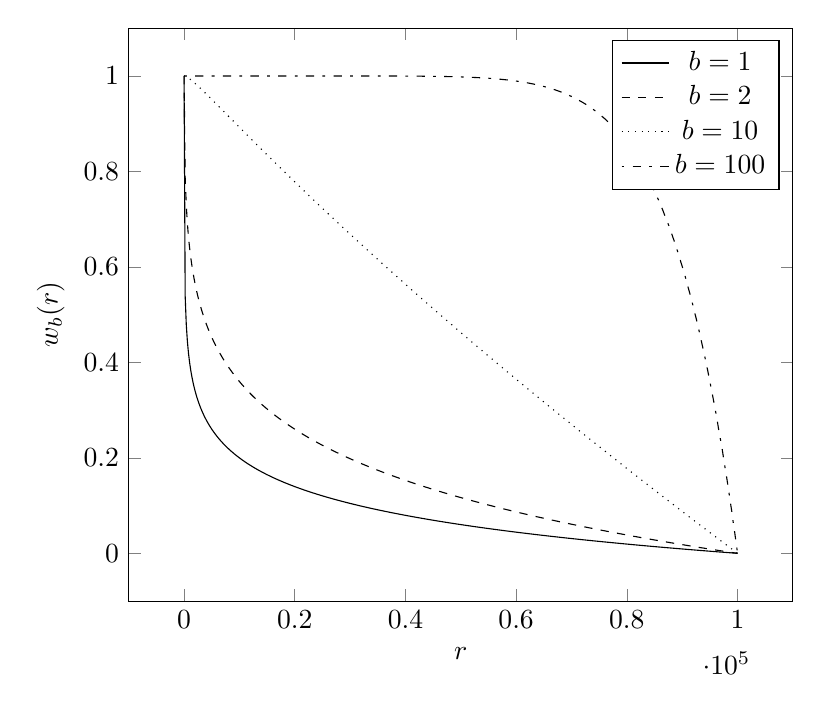
\begin{tikzpicture}
  
      \pgfplotsset{
          scale only axis,
      }
  
      \begin{axis}[
          xlabel=$r$,
          ylabel=$w_b(r)$,
          samples=500,
          ]
          \addplot[][domain=1:100000]{1-pow(ln(x*100000) / ln(100000) - 1., 1)};
          \addlegendentry{$b=1$}
          \addplot[style=dashed][domain=1:100000]{
              1-pow(ln(x*100000) / ln(100000) - 1., 2)};
          \addlegendentry{$b=2$}
          \addplot[style=dotted][domain=1:100000]{1-pow(ln(x*100000) / ln(100000) - 1., 10)};
          \addlegendentry{$b=10$}
          \addplot[dash pattern=on 1pt off 3pt on 3pt off 3pt][domain=1:100000]{1-pow(ln(x*100000) / ln(100000) - 1., 100)};
          \addlegendentry{$b=100$}
      \end{axis}
  
      \end{tikzpicture}
    }
    \captionof{figure}{Weighting factor $w_b$ plotted for several values of $b$}
    \label{fig:weightingfactor}
  \end{minipage}%
\end{figure}

It is noteworthy that a change of $b$ will also affect the average magnitude of the loss and thereby the effective step size. When comparing different weighting factors with each other, the loss term should therefore be divided by
\begin{equation}\label{eq:losswnormalization}
\frac{2}{r_\text{max}}\int_1^{r_\text{max}}w_b(r)dr\,,
\end{equation}
which evaluates to $\approx0.95$ for $b=10$ and $\approx0.17$ for $b=1$. Intuitively, the loss must be scaled up more (divided by a lower value) if the area under curve is lower. For $b=1$ it is lower than it is e.g. for $b=10$ (see Figure~\ref{fig:weightingfactor}).

During training, the gradient induced by the loss term (Equation~\ref{eq:loss}) can be approximated with fewer than $N$ samples, so called mini-batches. This is less costly than computing the gradient for the exact problem and has a regularizing effect, see \cite{DBLP:journals/corr/KeskarMNST16}.

Note that this is single scalar supervision (or binary classification) and it effectively trains a CNN plus GN successfully.

\subsection{Accuracy and Inference}
\label{sec:accuracy}

During training we evaluate the performance of our model by computing an \textbf{accuracy} metric. Given all possible $N\times N$ pairs of samples in the dataset, the accuracy is the percentage of pairs the model ranks correctly. It is defined as \begin{equation}\label{eq:acc}
    \frac{1}{N^2-N}\left(\sum_{i=1}^N\sum_{j=1}^N\bm{1}\left[\left(O_{i,j}<0\land P_{i,j}=0\right)\lor\left(O_{i,j}>0\land P_{i,j}=1\right)\right]\right)\,,
\end{equation}with $\bm{O}$ being the output matrix (defined in Equation~\ref{eq:outputmatrix}) and $\bm{P}$ being the ground truth (defined in Equation~\ref{eq:groundtruthmatrix}). $\bm{1}\left[\cdot\right]$ is $1$ if the boolean expression enclosed in the brackets is true, $0$ otherwise. The additional $(-N)$ term in the denominator of the leading normalization factor accounts for the main diagonal of the matrix which is always correctly ranked because $O_{i,i}=0$, so we disregard it. For performance purposes the symmetric property of the matrix may be exploited. The evaluation of the lower triangular part suffices to compute the accuracy score with adjusted normalization factor.

Verbally described, the accuracy measure is the percentage of correct pairwise rankings. It is easy to interpret and can be computed for humans as well, by showing them the sample pairs and requesting a ranking.

The accuracy evaluation metric has the downside of not taking the difficulty into consideration: Ranking e.g. sample \#55000 relative to sample \#54590 is presumably much harder than samples \#100 and \#40000, because the sample ranks are closer together.

In our setup, \textbf{inference} can be done in two ways: (1) absolute and (2) relative. In our experiments we do not need the rank inference mode (1) because the accuracy on validation and test set can be computed with Equation~\ref{eq:acc}. We present both modes anyways for use in future research or in applications. The two methods differ in that (1) requires the ground truth dataset $\mathbb{D}$, whereas (2) works with any set of two or more websites.

\begin{enumerate}
    \item[(1)] A single sample $G$ can be ranked with respect to the samples of the dataset $\mathbb{D}$. This can be done by computing $f_G=f_\text{model}(G)$ and comparing it to all entries in the vector $\bm{f}$. The estimated rank of $G$ is \begin{equation}
        \label{eq:inference}
        r^{(G)}\approx N-\sum_{i=1}^N\bm{1}\left[f_G>f_i\right]\,.
    \end{equation}
    \item[(2)] The relative inference compares a set of samples $\mathbb{S}$ relative to each other, where $\left\lvert\mathbb{S}\right\rvert\ge2$. Instead of computing the matrix $\bm{O}$ for samples in the dataset we compute it for $\mathbb{S}$. The entry at $O_{i,j}$ indicates how the samples with index $i$ and $j$ are ranked relative to each other.
\end{enumerate}
